\chapter{Blockchain as the Infrastructure of Semantic Web}
A distributed ledger is increasingly used to represent transactions between multiple parties throughout the world. It is difficult to search for specific information in a distributed ledger without an index. Therefore, indexing data in the distributed ledger is a requirement that provides the ability to search across multiple ledgers, enhancing the power and usability of this system as well \cite{Third}.
\section{Distributed Ledgers and Indexing}
A distributed ledger based on a blockchain does not have central control. Blockchains are organized into multiple blocks; the initial block is created manually, and the other blocks are added by some consensus process between nodes.
The Ethereum smart contract provides the possibility to automatically control what happens with cryptocurrency on the blockchain without involving untrusted external sources. Ethereum smart contracts have an account that can normally store, update, or perform a function with the input and output.
As smart contracts are time-ordered, where data are stored in blocks, the data must be indexed. Indexing the smart contract gives us the capability to access the data, search, analyze services on the distributed ledger, and expose them to the outside world for more interactions.
There are different levels of indexing smart contracts: The basic level is the fundamental level for the next step. It indexes basic entities such as accounts and blocks related to distributed levels, and data can be stored or retrieved here. At the functional level, smart contracts contain a lot of functional interfaces that depict the other functionality of platforms such as Ethereum \cite{Third}.
\subsection{Why Do We Use Ontology for Blockchain?}
Generally, blockchain is a distributed database that is replicated over all nodes and uses a cloud computing architecture. In the other word, data in database distributed across many organizations. Thus, data should have a common interpretation to be understandable for organizations. These interpretations are applicable via a formal specification that enables verification and inference within software and applications executed on the network. \\
This is where ontology plays the main role in ensuring a common interpretation of data in the shared database among different enterprises.
Blockchain as a modeling form uses a different type of ontology \cite{Kim}: \\
\\
\textbf{\textit{Informal/Semi ontology}} facilitates search and enhances a better understanding of the business process for developing and applying on the blockchain \cite{Kim}. \\
\\
\textbf{\textit{Formal ontology}} helps the formal specification automate inference and verify the operation of the blockchain. In other words, blockchain modeling based on a formal ontology can help with the development of smart contracts to execute on the blockchain \cite{Kim}. \\
\\
Also, we can use ontologies to capture data within the blockchain: On the one hand, it facilitates a better understanding of blockchain concepts for humans. On the other hand, it enables interlinking with other linked data to convey deductions and formal reasoning \cite{Kim}.\\
Vocabulary used within an ontology increases the transparency of transactions by describing the transaction in the context of linked data and facilitating the graphical representation of the location of such transactions. Thus, it also increases the capability of analysis by users \cite{Kim}.

\begin{center}
	
	
	\begin{figure}[htb!]
		
		\begin{minipage}{0.55\linewidth}
			\centering
			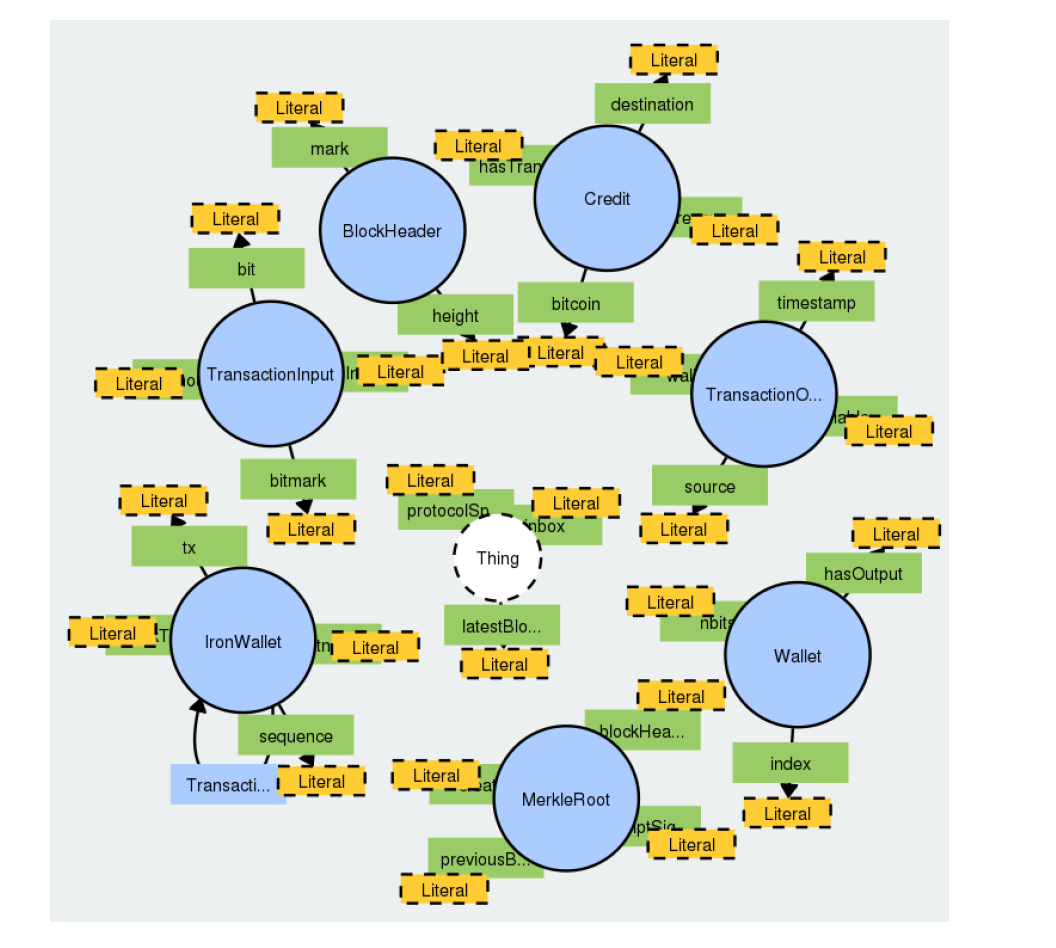
\includegraphics[width=1.65\textwidth]{images/chap02_diagram_ontology.png}
		\end{minipage}
		\caption[Illustration of ontology diagram]{Illustration of ontology diagram \cite{Matthew}}
		
		
	\end{figure}
	
\end{center}

\subsection{Linked Data}
According to Tim Berbers-Lee et al. \cite{Tim}, 'Linked data is about using the Web to create typed links between data
from different sources'. When information
is presented as linked data, other related information can be easily retrieved, and new information can also be easily linked to it. \textit{Berners-Lee} described four rules for linked data:\\
\textbf{- URIs} (Uniform Resource identifier) as names.\\
\textbf{- HTTP} to search for names.\\
\textbf{- (SPARQL, RDF)} provides related information about what a user looking for. \\
\textbf{- Link} to other URLs to provide more information \cite{Hector}.\\

\begin{center}
	\begin{figure}[htb!]
		
		\begin{minipage}{0.55\linewidth}
			\centering
			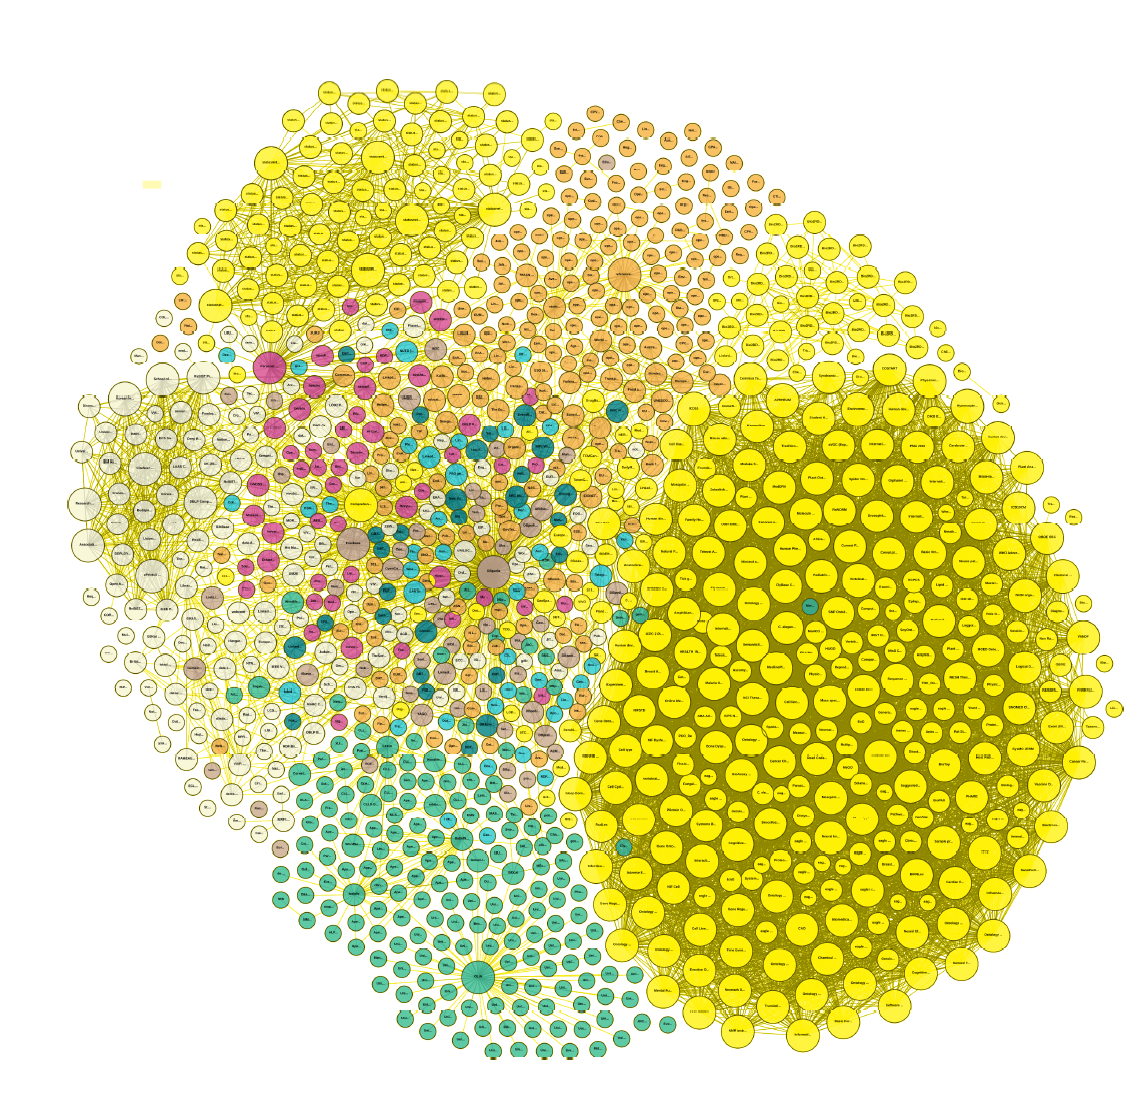
\includegraphics[width=1.55\textwidth]{images/chap02_LinkData.png}
		\end{minipage}
		\caption[Linked data diagram]{Linked data diagram \cite{Hector}}
		
		
	\end{figure}
	
\end{center}
\subsection{RDF}
The Resource Description Framework (RDF) is a family of W3C specifications. RDF is used to describe and model information. It describes a subject that predicts an object and is called a triple.
i) Subjects that RDF expressions describe.
ii) Predict specific properties, attributes, or relationships to describe a resource.
iii) The object is the name of a property or value \cite{Hector}.
\subsection{SPARQL}
According to Wikipedia's definition, "it is a semantic query language for a dataset that makes us able to retrieve and modify data stored in RDF format known as triples.". SPARQL can query the one, two, or all elements of triples.

\subsection{OWL (Ontology Web Language) }
Ontology web language is made to represent knowledge about things and the relations among them. OWL is a computational logic-based language, which means the language modeled in OWL can operate in a computer program like negation, intersection, and so on \cite{Hector}.
\subsection{Evolution of World Wide Web}
The evolution and interaction of people on the Internet are classified based on three technologies: \\
\begin{itemize}
\item\textit{Web 1.0} also known as \textit{web of document} is the earliest website with the basic capability of linking to other websites. \\
\item\textit{Web 2.0} known as \textit{web of data} has the capability of providing space for users to collaborate on content creation or modification.\\
\item\textit{Web 3.0} is strengthened by the semantic web, where people have access to linked information on the web. But recently, with the arrival of distributed technologies like blockchain and Ethereum which get used by Web 3.0, this is a new focus on this \cite{Kujur}.
\end{itemize}

\section{Vocabularies}
\subsection{Vocabulary in Distributed Ledger}
Generating linked data requires the use of a standard ontology or vocabulary to explain blockchain concepts. Interfaces between distributed ledgers and the semantic web are still in their early stages. There are some systems and vocabularies that specify such a vocabulary
like FlexLedger, EthOn, and BLONDiE. \cite{Third}.\\
\\
\textbf{\textit{FlexLedger}} describes HTTP interfaces to blockchains, with a standard vocabulary and responses to these interfaces. It is a protocol for decentralized ledger and graph data models that represent ledger creation, querying, and data modeling using JSON-LD. However, FlexLedger does not have an explicit vocabulary about ontology, nor does it have a concrete ontology for itself. \\
It is striking to say that the FlexLedger is not suitable to implement in some graph models like graph chains because in the FlexLedger meta and the content data are stored together in the same graph, whereas the GraphChain blocks content is stored outside the blockchain in a separate graph \cite{Sopek}.\\
\\
\textbf{\textit{EthOn}} is an OWl ontology that describes blockchain classes such as \textit{'blocks', 'accounts', 'message', 'state'} and relations such \textit{'has parent block'} \cite{Rashid}. 
\begin{center}
	
	\begin{figure}[htb!]
		
		\begin{minipage}{0.50\linewidth}
			\centering
			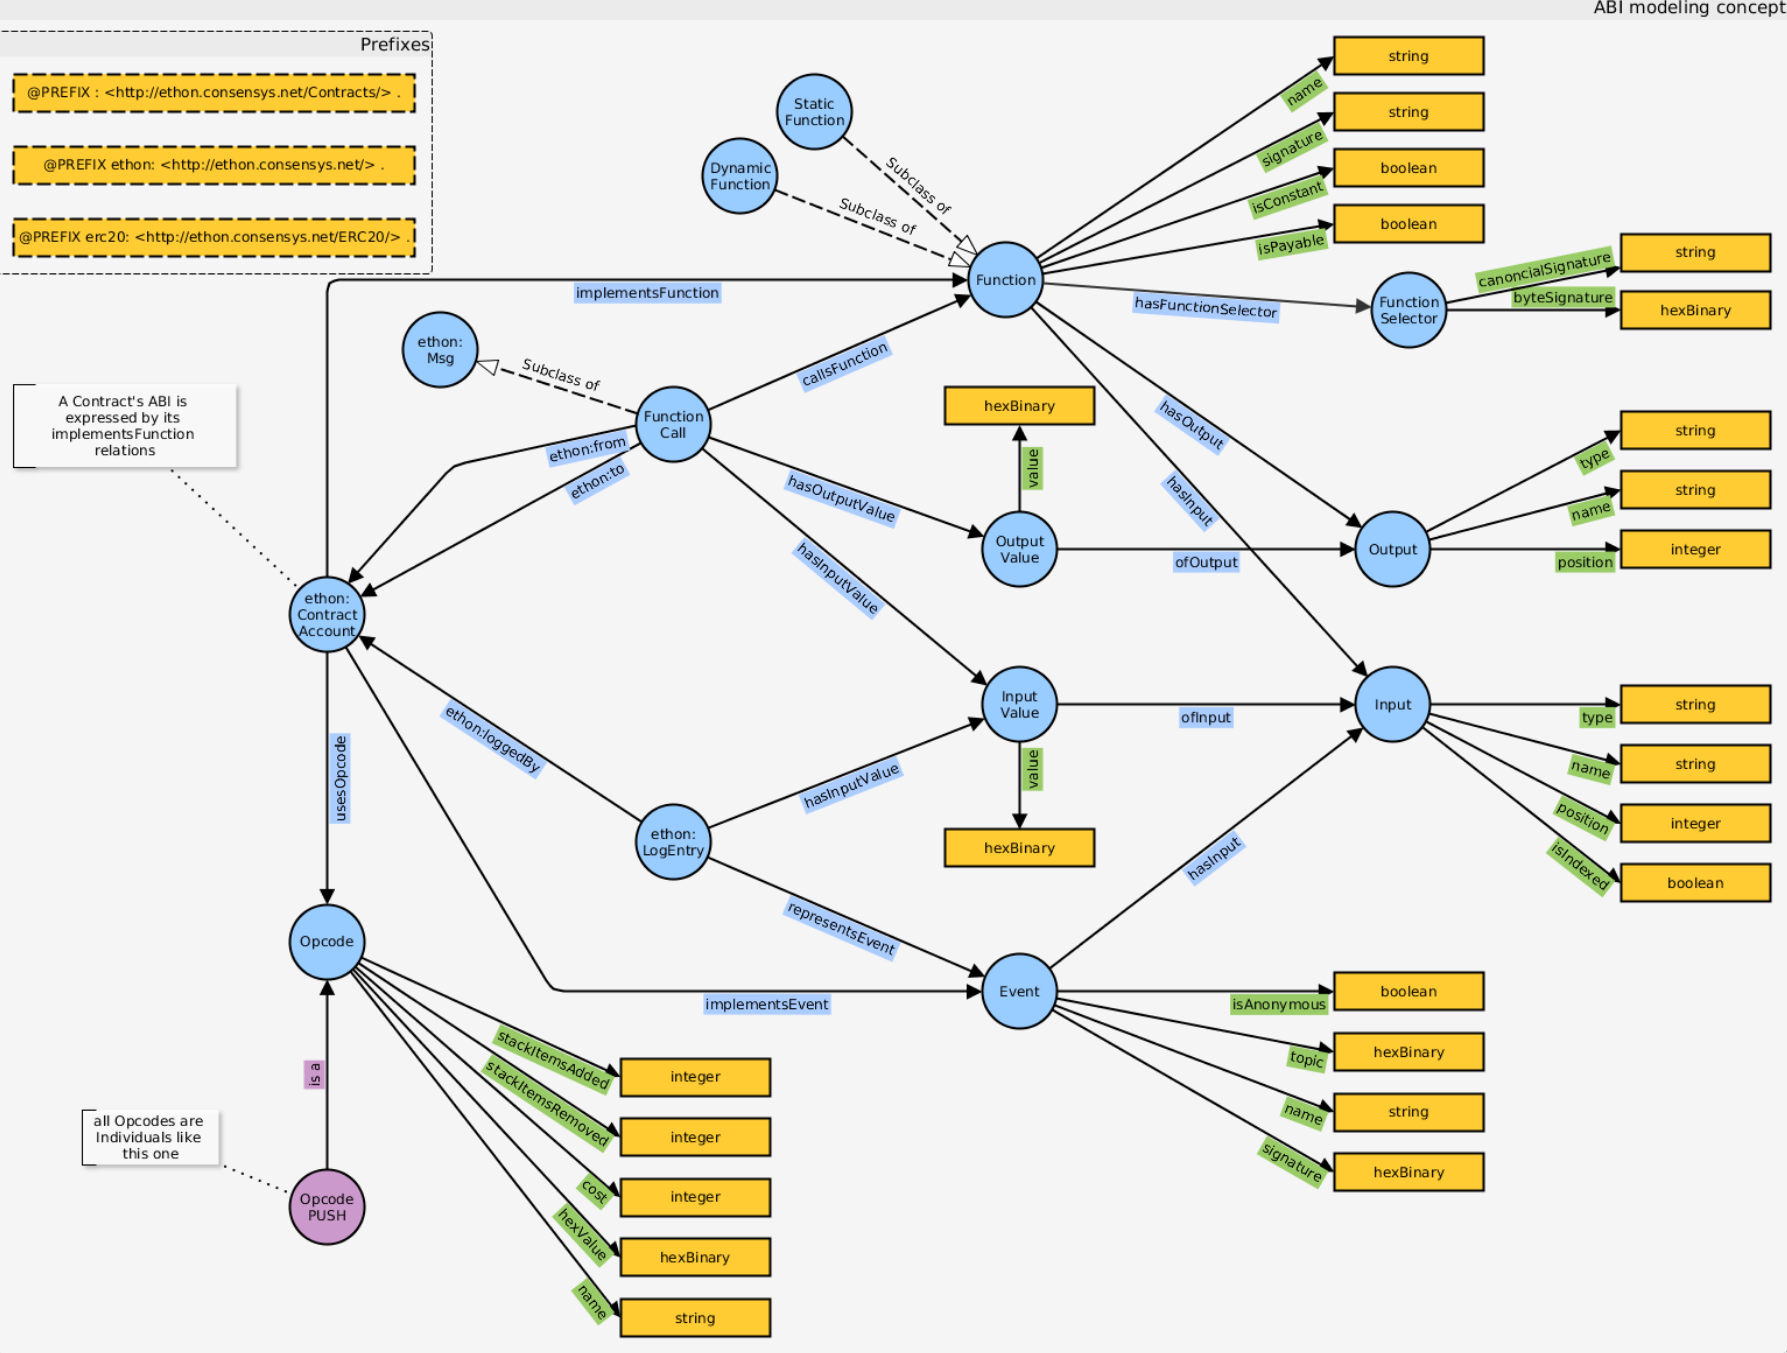
\includegraphics[width=1.80\textwidth]{images/chap2_EthOnContract.png}
		\end{minipage}
		\caption[EthOn classes]{EthOn contract model(blue arrow is object properties, green arrow is data properties, purple circle is instance and blue one is class) \cite{Rashid}}
		
	\end{figure}
	
	\begin{figure}[htb!]
		
		\begin{minipage}{0.55\linewidth}
			\centering
			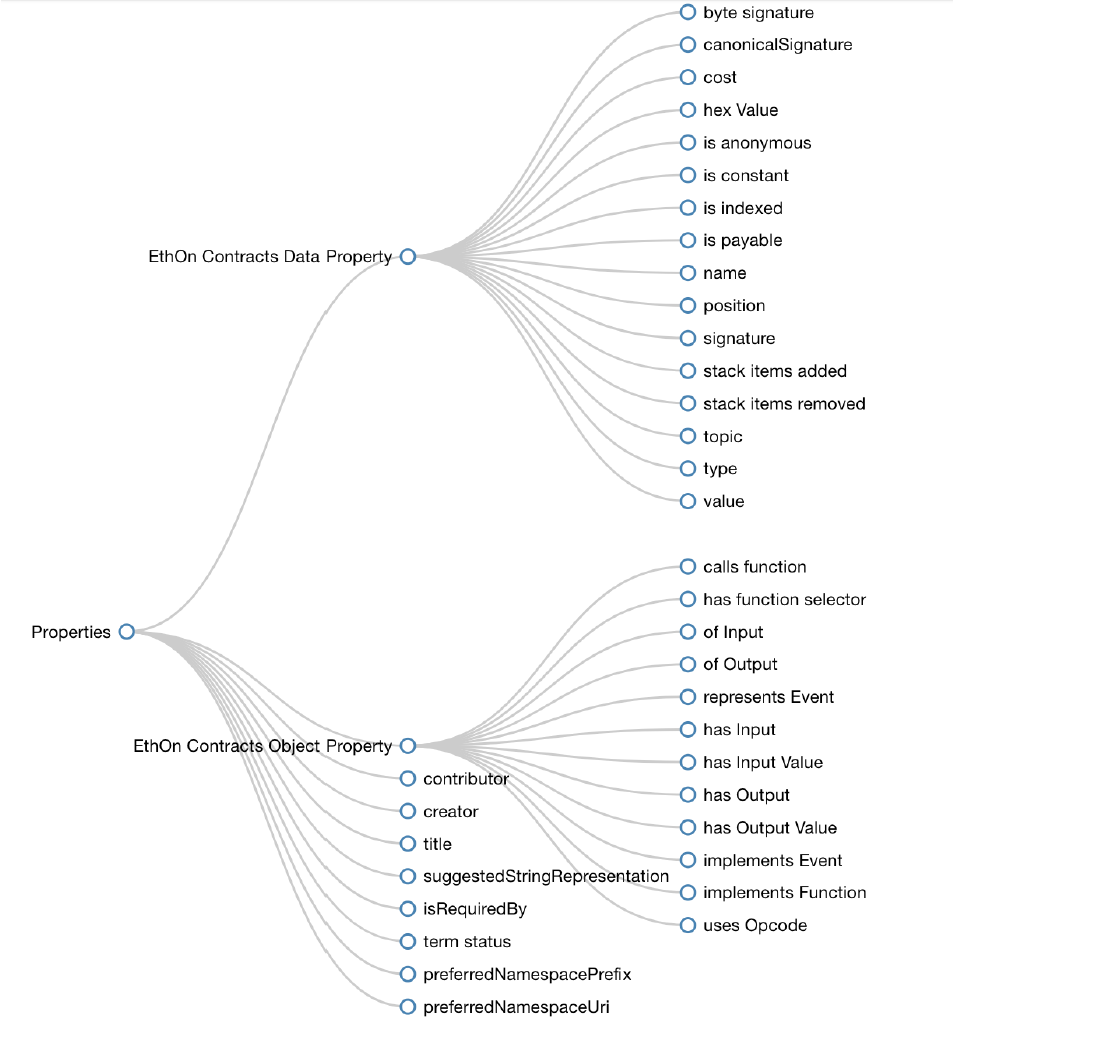
\includegraphics[width=1.65\textwidth]{images/chap02_EthOn_Properties.png}
		\end{minipage}
		\caption[EthOn properties]{EthOn properties \cite{Rashid}}
		
		
	\end{figure}
	
\end{center}
\textbf{\textit{BLONDiE (Blockchain Ontology with Dynamic Extensibility)}} is another OWL ontology for describing the blockchain structure, like EthOn. But it is more generic than EthOn. For example, EthOn and BLONDiE both defined some terms such as 'account', 'block', and 'transaction', as well as some attributes such as 'transaction payload' or 'miner address'. BLONDiE defines some other concepts for different blockchains, such as 'BitcoinBlockHeader' and 'EthereumBlockHeader' as subclasses of 'BlockHeader'. At the moment, BLONDiE supports two cryptocurrencies like bitcoin and Ethereum, where all links and relations between objects and attributes are represented in RDF (Resource Description Framework) \cite{Third}.
\begin{center}
	\begin{figure}[htb!]
		
		\begin{minipage}{0.55\linewidth}
			\centering
			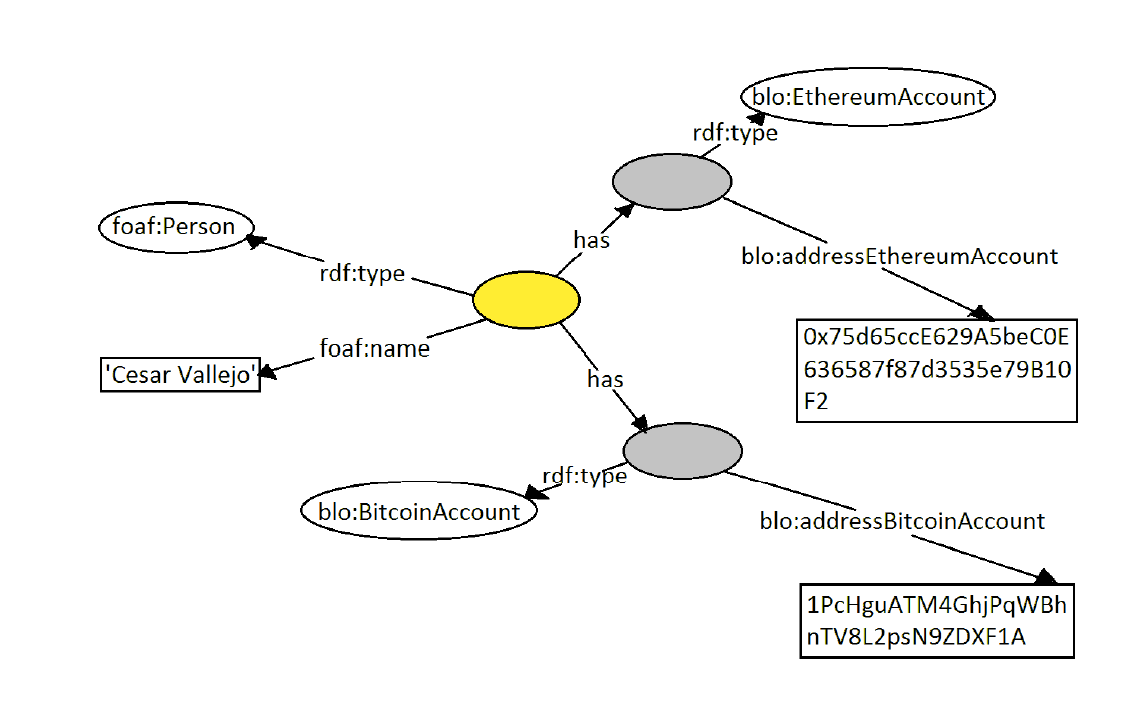
\includegraphics[width=1.75\textwidth]{images/chap02_BLONDiE.png}
		\end{minipage}
		\caption[BLONDiE]{BLONDiE usage example \cite{Hector}}
		
		
	\end{figure}
	
\end{center}
\subsection{Vocabulary in Smart Contract}
As mentioned earlier, EthOn and BLONDiE are both similar concepts that can be used for smart contracts. There are many works on semantic annotation of the web and HTTP-APIs that may enable us to annotate smart contracts as well. However, the contracts are not web APIs, and the implementation may differ, but the main concept does not. In other words, the vocabularies used to annotate web services are also used to annotate smart contracts. It seems that the combination of a distributed ledger with a smart contract and web service due to profitability will become common \cite{Third}.

\section{Semantify Blockchain}
\subsection{Semantic Blockchain}
With increasing the use of blockchain technology recently, the need for semantic reasoning on the distributed ledger is on the increase as well. The blockchain is the best platform to utilize semantic web principles in this technology and add a new trusted property to a dataset. 
Using semantic web technology on the blockchain is a novel idea and the way how to apply this technology in blockchain and smart contracts is also a controversial issue.\\
There are some \textbf{definition of semantic blockchain:}\\ 
\textit{- Semantic blockchain is the representation of stored data on distributed ledger using linked data. }\\
\textit{- Semantic blockchain is the applying semantic web standard on the blockchain that these standards are based on RDF \cite{Hector}.}
\subsection{Semantification Process}
Semantic blockchain or semantic distributed ledger affects the industrial world and subsequently, the result leads to the start development of new applications and frameworks to combine two worlds.
there are some ways to semantify blockchain as bellow:\\
\textbf{-} Mapping the blockchain data to RDF making usage of vocabulary, ontology, and so on. \\
\textbf{-} Storage of data in a blockchain is expensive, The only way is to store the hashing point to the data set in the blockchain and then share RDF on the blockchain. \\
\textbf{-} Creating semantic blockchain that exchanges internal data protocol in RDF format \cite{Hector}. \\
\subsection{Semantic Ontology Mapping using BLONDiE} 
To generate RDF, it needs to map the basic blockchain entities to relevant semantic web terms, concepts, and ontologies. To make the query more efficient, BLONDiE is extended in two ways: Firstly, records relating to both blocks and transactions have been
augmented with an attribute for the hash of each entity. Secondly, records relating to the transactions have been augmented with links to entities like blocks or smart contracts.\\
Blockchain stores just a binary form of each contract with metadata. To interact with the contract, the Application Binary Interface (ABI) specification is required. This specification is in the form of JSON and is created when a smart contract is compiled and stored on the blockchain. The ABI determines all functions of contracts and provides descriptions of input, and output parameters for each contract \cite{Third}.

\begin{center}
	\begin{figure}[htb!]
		
		\begin{minipage}{0.45\linewidth}
			\centering
			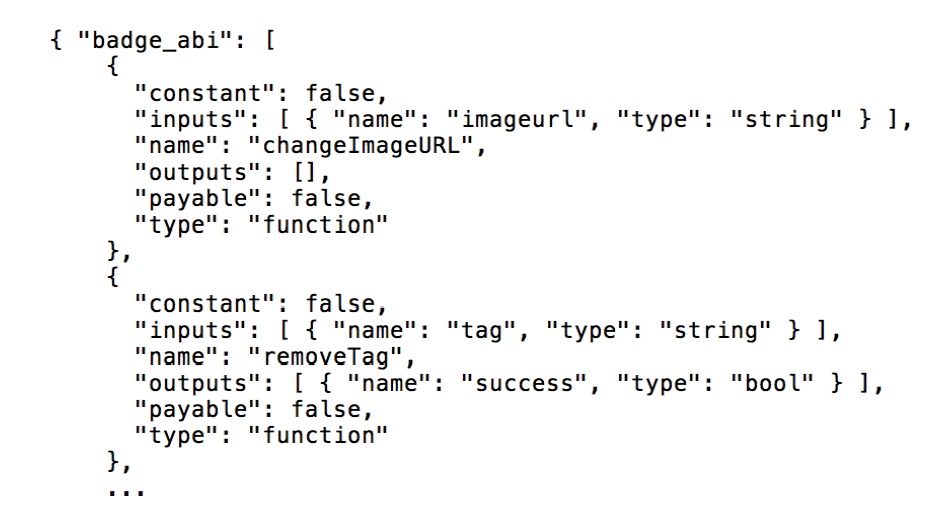
\includegraphics[width=1.95\textwidth]{images/chap02_SmartContract_ABI.png}
		\end{minipage}
		\caption[Smart contract application binary interface (ABI)]{Smart contract application Bbinary interface (ABI)}
		
	\end{figure}
	
\end{center}